\documentclass{beamer}
\usetheme{Warsaw}

\usepackage{amsfonts} % math symobls
\usepackage{amsthm}
\usepackage[utf8]{inputenc}
\usepackage{polski}
\usepackage{graphics}
\usepackage{verbatim}

\newcommand{\emp}[1]{\textcolor{blue}{\textit{#1}}}
\newcommand{\red}[1]{\textcolor{red}{#1}}

\title{Rozpoznawanie chorób skóry}
\author{Michał Karpiński}
\date{24 stycznia, 2013}

\begin{document}

\begin{frame}[plain]
  \titlepage
\end{frame}

\begin{frame}{Choroby skóry}

       1             psoriasis(łuszczyca)	     112
       2             seboreic dermatitis(łojotokowe zapalenie skóry)             61
       3             lichen planus(liszaj płaski)    72
       4             pityriasis rosea (łupież różowy Giberta)                49
       5             chronic dermatitis (atopowe zapalenie skóry)               52    
       6             pityriasis rubra pilaris (Rogowacenie przymieszkowe czerwone)       20

Clinical Attributes: (take values 0, 1, 2, 3, unless otherwise indicated)
      1: erythema
      2: scaling
      3: definite borders
      4: itching
      5: koebner phenomenon
      6: polygonal papules
      7: follicular papules
      8: oral mucosal involvement
      9: knee and elbow involvement
     10: scalp involvement
     11: family history, (0 or 1)
     34: Age (linear)

Histopathological Attributes: (take values 0, 1, 2, 3)
     12: melanin incontinence
     13: eosinophils in the infiltrate
     14: PNL infiltrate
     15: fibrosis of the papillary dermis
     16: exocytosis
     17: acanthosis
     18: hyperkeratosis
     19: parakeratosis
     20: clubbing of the rete ridges
     21: elongation of the rete ridges
     22: thinning of the suprapapillary epidermis
     23: spongiform pustule
     24: munro microabcess
     25: focal hypergranulosis
     26: disappearance of the granular layer
     27: vacuolisation and damage of basal layer
     28: spongiosis
     29: saw-tooth appearance of retes
     30: follicular horn plug
     31: perifollicular parakeratosis
     32: inflammatory monoluclear inflitrate
     33: band-like infiltrate

\end{frame}

%\begin{center}
%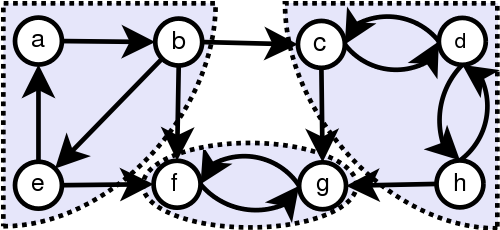
\includegraphics[scale=0.5]{img/Scc.png}
%\end{center}

\end{document}
